\documentclass[a4paper]{article}

\usepackage[T1]{fontenc}
\usepackage[portuguese]{babel}
\usepackage{hyphenat}

\usepackage{geometry}
 \geometry{
 a4paper,
 left=20mm,
 right=20mm,
 top=30mm,
 bottom=20mm,
 }

\usepackage{fancyhdr}
\pagestyle{fancy}
\rhead{Bruno Corrêa Zimmermann -- 313985}
\title{Paginação de Memória, TLB, e Localidade -- Estudo de Caso}
\author{Bruno Corrêa Zimmermann}
\date{20 de Abril de 2022}
\setlength{\headheight}{13pt}

\usepackage{placeins}
\usepackage{amssymb}
\usepackage{enumitem}
\usepackage{upquote}
\usepackage{amsmath}
\usepackage{fancyvrb}
\usepackage{tgcursor}
\usepackage{fancyvrb}
\usepackage{minted}
\usepackage{xcolor}
\usepackage{graphicx}
\usepackage{biblatex}
\usepackage{csquotes}
\addbibresource{trab2.bib}
\definecolor{LightGray}{gray}{0.9}
\renewcommand{\baselinestretch}{1.5}
\newenvironment{code}[1]{
\VerbatimEnvironment
\begin{minted}[frame=single,baselinestretch=1,fontsize=\small]{#1}}{
\end{minted}
}

\begin{document}

%\fontsize{12}{12}
%\selectfont

\maketitle

NOTA: os códigos se encontram no repositório
https://github.com/brunoczim/sisop1-trab2

\section{Introdução}

Memória virtual é um mecanismo de abstração da memória física que dá a impressão
a um processo de que o espaço de memória onde ele está pertence todo a ele. Uma
forma de implementar esse mecanismo, usada em processadores x86-64, em sistemas
como Linux, é paginação de memória. Nesse sistema, a memória é dividida em
páginas de tamanho fixo, e, no caso de Linux x86-64, o tamanho é 4KiB.

Nesse esquema, há páginas virtuais e páginas físicas. Páginas virtuais são
mapeadas para páginas físicas, mas processos enxergam apenas as páginas
virtuais. Para realizar a tradução entre endereços, é necessário manter tabelas
de páginas. As páginas virtuais podem não estar mapeadas ainda, e nesse caso,
ao tentar acessá-las, o processador gera um sinal chamado
``\textit{Page Fault}'', e então o sistema operacional mapeia a página virtual
para uma página física.

É possível que uma página seja armazenada em disco. Quando um processo tenta
acessar um endereço virtual, busca-se na tabela de páginas a entrada da página
virtual do endereço. Se não está mapeada (\textit{bit} de validade valendo $0$),
busca-se do disco a página e define-se o \textit{bit} de validade para $1$. Em
ambos os casos, ao final, obtém-se o número da página física, e dentro dela, o
enedereço físico é acessado.

Na tabela de páginas, há alguns \textit{bits} de controle para cada entrada.
O \textit{bit} mencionado acima (\textit{bit} de validade) indica se a entrada
na tabela é válida, ou seja, se há um mapeamento válido para a página virtual
associada à entrada. Há ainda o \textit{bit} ``\textit{dirty}'', que indica se a
página física associada àquela entrada na tabela está incosistente com o disco,
e no caso de substituição LRU (\textit{Least Recently Used}), um bit de
referência, indicando se essa entrada foi usada recentemente.

A tabela de páginas é finita, e portanto, quando uma nova página precisa ser
carregada, é possível que outra precise ser descarregada. Existem várias formas
de definir quais páginas serão descarregadas, e o LRU é um algoritmo que resolve
esse problema, substituindo as páginas que foram usadas pela última vez há mais
tempo. Outro algoritmo é o FIFO (\textit{First-in, First-out}), que substitui a
página carregada há mais tempo.

Além da tabela de páginas, existe um \textit{cache} de páginas, chamado TLB
(\textit{Translation-Lookaside Buffer}). O TLB se assemelha a tabela de
páginas convencional, mas é implementado em \textit{hardware}, então, se uma
página está no TLB, faz-se apenas um acesso à memória, em comparação aos
dois acesso pela tabela de página tradicional. Como é um \textit{cache}, ele não
armazena a estrutura toda das tabelas de páginas, mas apenas páginas
específicas, e portanto a TLB também guarda uma \textit{tag} para identificar a
página guardada em uma entrada.

Portanto, para aproveitar a performance do TLB, ou até mesmo da tabela de
páginas convencional, é importante que os programas busquem ter boa localidade.
Por exemplo, sequências de endereços que ``pulam'' páginas podem acabar fazendo
mau uso da TLB. Neste artigo, vamos estudar os efeitos de usar-se diferentes
estruturas de dados, com diferentes algoritmos, e com diferentes localidades.

\section{Localidades e Programas Estudados}

Para explorar efeitos de localidade sobre a TLB, foram experimentadas três
estruturas de dados: \textit{arrays}, árvores binárias, e listas simplesmente
encadeadas. No entanto, para \textit{arrays}, foram usados quatro algorimtos de
busca diferentes: busca binária (\textit{sorted-array}), busca linear com boa
localidade (\textit{good-local-array}), busca linear com má localidade
(\textit{bad-local-array}) e busca linear com localidade péssima
(\textit{worse-local-array}).

Para árvores binárias, dois algoritmos foram usados: uma busca assumindo que a
árvore está ordenada (\textit{with-order-tree}), padrão de árvores de busca, e
uma busca que não assume isso (\textit{without-order-tree}). Sobre a lista
encadeada, foi usado apenas um algoritmo de busca linear (\textit{linked-list}).

Para cada estrutura de dados foram testadas duas operações: busca
(\textit{find}) e incremento de todos elementos menores que um certo valor
(\textit{inc-less-than}). A operação \textit{find} busca o elemento e retorna
um valor informando se o elemento foi encontrado, enquanto a operação
\textit{inc-less-than} de fato incrementa todos elementos menores que um dado
valor. Na figura \ref{fig:good local array find}, vemos a implementação da
operação \textit{find} para \textit{good-local-array}: é uma simples busca
linear e percorre pelos elementos em ordem, endereço após endereço.

\begin{figure}
    \begin{code}{Rust}
pub fn find_good_local(&self, element: ElementType) -> bool {
    let mut i = 0;
    while i < self.elements.len() {
        if self.elements[i] == element {
            return true;
        }
        i += 1;
    }
    false
}
    \end{code}
    \caption{Implementação da operação \textit{find} para
        \textit{good-local-array}}
    \label{fig:good local array find}
\end{figure}

A implementação da operação \textit{find} para \textit{bad-local-array} está na
figura \ref{fig:bad local array find}, que ao invés de percorrer em ordem, testa
o primeiro elemento da primeira página do \textit{array}, e então testa o
primeiro elemento da décima sexta página, então o primeiro elmento da trigésima
segunda página, até testar o primeiro elemento de cada grupo de dezesseis
páginas. Depois disso, ele testa o segundo elemento de cada grupo, e então
o terceiro, até que o último elemento de cada grupo seja testado. A expectativa
é que essa implementação pule páginas com muita frequência e force o TLB a
substituir páginas.

\begin{figure}
    \begin{code}{Rust}
pub fn find_bad_local(&self, element: ElementType) -> bool {
    let jump_pages = 16;
    let jump_elements = jump_pages * ELEMS_IN_PAGE;
    let mut offset = 0;
    while offset < jump_elements {
        let mut jump_page = 0;
        let mut index = jump_page * jump_pages + offset;
        while index < self.elements.len() {
            if self.elements[index] == element {
                return true;
            }
            jump_page += 1;
            index = jump_page * jump_pages + offset;
        }
        offset += 1;
    }
    false
}
    \end{code}
    \caption{Implementação da operação \textit{find} para
        \textit{bad-local-array}}
    \label{fig:bad local array find}
\end{figure}

O código na figura \ref{fig:worse local array find} implementa essa operação
para \textit{worse-local-array}, que, em teoria, teria localidade pior do que
\textit{bad-local-array}. Essa implementação, além de pular dezesseis páginas,
divide o \textit{array} em dois, e intercala entre as duas metades: primeiro
testa um elemento da primeira metade, depois testa um elemento da segunda
metade, sempre pulando dezesseis páginas em cada metade.

\begin{figure}
    \begin{code}{Rust}
pub fn find_worse_local(&self, element: ElementType) -> bool {
    let rounded = self.elements.len() + ELEMS_IN_PAGE - 1;
    let pages = rounded / ELEMS_IN_PAGE;
    let half_size = pages / 2 * ELEMS_IN_PAGE;
    let jump_pages = 16;
    let jump_elements = jump_pages * ELEMS_IN_PAGE;
    let mut offset = 0;

    while offset < jump_elements {
        let mut jump_page = 0;
        let mut in_bounds = true;
        let mut index = jump_page * jump_pages + offset;
        while in_bounds {
            in_bounds = false;
            let lower_index = index;
            if lower_index < half_size {
                if self.elements[lower_index] == element {
                    return true;
                }
                in_bounds = true;
            }
            let upper_index = index + half_size;
            if upper_index < self.elements.len() {
                if self.elements[upper_index] == element {
                    return true;
                }
                in_bounds = true;
            }
            jump_page += 1;
            index = jump_page * jump_pages + offset;
        }
        offset += 1;
    }

    false
}
    \end{code}
    \caption{Implementação da operação \textit{find} para
        \textit{worse-local-array}}
    \label{fig:worse local array find}
\end{figure}

As implementações da operação \textit{inc-less-than} para esses três tipos de
\textit{array} (\textit{good-local-array}, \textit{bad-local-array},
\textit{worse-local-array}) seguem o mesmo princípio que as implementações da
operação \textit{find}, exceto que dessa vez ao invés de buscar um certo
elemento, buscam elementos menores que um certo valor e incrementam tais
elementos. Observe, nas figuras \ref{fig:good local array inc less than},
\ref{fig:bad local array inc less than} e
\ref{fig:worse local array inc less than}, que o \textit{array} é percorrido da
mesma forma que na operação \textit{find}, mas dessa vez é por todo o
\textit{array}.

\begin{figure}
    \begin{code}{Rust}
pub fn inc_less_than_good_local(&mut self, element: ElementType) {
    let mut i = 0;
    while i < self.elements.len() {
        if self.elements[i] < element {
            self.elements[i]+= 1;
        }
        i += 1;
    }
}
    \end{code}
    \caption{Implementação da operação \textit{inc-less-than} para
        \textit{good-local-array}}
    \label{fig:good local array inc less than}
\end{figure}

\begin{figure}
    \begin{code}{Rust}
pub fn inc_less_than_bad_local(&mut self, element: ElementType) {
    let jump_pages = 16;
    let jump_elements = jump_pages * ELEMS_IN_PAGE;
    let mut offset = 0;

    while offset < jump_elements {
        let mut jump_page = 0;
        let mut index = jump_page * jump_pages + offset;
        while index < self.elements.len() {
            if self.elements[index] < element {
                self.elements[index] += 1;
            }
            jump_page += 1;
            index = jump_page * jump_pages + offset;
        }
        offset += 1;
    }
}
    \end{code}
    \caption{Implementação da operação \textit{inc-less-than} para
        \textit{bad-local-array}}
    \label{fig:bad local array inc less than}
\end{figure}

\begin{figure}
    \begin{code}{Rust}
pub fn inc_less_than_worse_local(&mut self, element: ElementType) {
    let rounded = self.elements.len() + ELEMS_IN_PAGE - 1;
    let pages = rounded / ELEMS_IN_PAGE;
    let half_size = pages / 2 * ELEMS_IN_PAGE;
    let jump_pages = 16;
    let jump_elements = jump_pages * ELEMS_IN_PAGE;
    let mut offset = 0;

    while offset < jump_elements {
        let mut jump_page = 0;
        let mut in_bounds = true;
        let mut index = jump_page * jump_pages + offset;
        while in_bounds {
            in_bounds = false;
            let lower_index = index;
            if lower_index < half_size {
                if self.elements[lower_index] < element {
                    self.elements[index] += 1;
                }
                in_bounds = true;
            }
            let upper_index = index + half_size;
            if upper_index < self.elements.len() {
                if self.elements[upper_index] < element {
                    self.elements[index] =
                        self.elements[index].wrapping_add(1);
                }
                in_bounds = true;
            }
            jump_page += 1;
            index = jump_page * jump_pages + offset;
        }
        offset += 1;
    }
}
    \end{code}
    \caption{Implementação da operação \textit{inc-less-than} para
        \textit{worse-local-array}}
    \label{fig:worse local array inc less than}
\end{figure}

Adicionalmente, há uma implementação de \textit{array} com busca binária
em um \textit{aray} ordenado, chamada de \textit{sorted-array}. As
implementações de \textit{find} e \textit{inc-less-than} para
\textit{sorted-array} se encontram na figura
\ref{fig:sorted array find inc less than}. A ideia de usar essa estrutura de
dados é: busca binária tem uma complexidade logaritma, melhor, em teoria, do que
a complexidade linear da busca dos outros \textit{arrays}. No entanto, a busca
binária não tem uma boa localidade, ela salta entre partes do \textit{array}.
Deseja-se testar se a complexidade compensa mesmo com localidade ruim, ou se a
localidade prejudicará significativamente a performance da busca binária.

\begin{figure}
    \begin{code}{Rust}
fn binary_search(&self, element: ElementType) -> Result<usize, usize> {
    let mut left = 0;
    let mut right = self.elements.len();
    while left < right {
        let mid = left + (right - left) / 2;
        match element.cmp(&self.elements[mid]) {
            cmp::Ordering::Less => right = mid,
            cmp::Ordering::Equal => return Ok(mid),
            cmp::Ordering::Greater => left = mid + 1,
        }
    }
    Err(left)
}

pub fn find_sorted(&self, element: ElementType) -> bool {
    self.binary_search(element).is_ok()
}

pub fn inc_less_than_sorted(&mut self, element: ElementType) {
    let mut upper_bound = match self.binary_search(element) {
        Ok(upper_bound) => upper_bound,
        Err(upper_bound) => upper_bound,
    };

    while upper_bound > 0 && self.elements[upper_bound - 1] >= element {
        upper_bound -= 1;
    }

    let mut index = 0;
    while index < upper_bound {
        self.elements[index] = self.elements[index].wrapping_add(1);
        index += 1;
    }
}
    \end{code}
    \caption{Implementação das operações \textit{find} e \textit{inc-less-than}
        para \textit{sorted-array}}
    \label{fig:sorted array find inc less than}
\end{figure}

Em relação a listas simplesmente encadeadas, o objetivo é observar efitos da
localidade de ter nodos alocados não necessariamente em sequência, ao invés de
ter elementos em endereços contíguos. A implementação de \textit{find}, na
figura \ref{fig:linked list find}, é uma busca linear que percorre pelos
elementos em sequência, assim como \textit{inc-less-than}, na figura
\ref{fig:linked list inc less than}. Note que há um potencial problema de
localidade nessa sequência, porque o nodo seguinte pode estar em um endereço
distante do nodo atual.

\begin{figure}
    \begin{code}{Rust}
pub fn find(&self, element: ElementType) -> bool {
    let mut this = self;
    while let Some(top) = &this.top {
        if top.data == element {
            return true;
        }
        this = &top.next;
    }
    false
}
    \end{code}
    \caption{Implementação da operação \textit{find} para
        \textit{linked-list}}
    \label{fig:linked list find}
\end{figure}

\begin{figure}
    \begin{code}{Rust}
pub fn inc_less_than(&mut self, element: ElementType) {
    let mut this = self;
    while let Some(top) = &mut this.top {
        if top.data < element {
            top.data += 1;
        }
        this = &mut top.next;
    }
}
    \end{code}
    \caption{Implementação da operação \textit{inc-less-than} para
        \textit{linked-list}}
    \label{fig:linked list inc less than}
\end{figure}

A respeito de árvores binárias, há um objetivo parecido com listas encadeadas:
os nodos da árvore podem estar em endereços distantes. Entretanto, também há o
objetivo de observar quanta vantagem há em aproveitar o fato de uma árvore estar
ordenada para buscas. Na figura \ref{fig:with order tree find}, está a
implementação da operação \textit{find} para árvores ordenadas
(\textit{with-order-tree}), que assume que nodos à esquerda contêm valores
menores do que o nodo atual, enquanto nodos à direita contêm valores maiores.

\begin{figure}
    \begin{code}{Rust}
pub fn find_with_order(&self, element: ElementType) -> bool {
    let mut this = self;
    while let Some(node) = &this.root {
        match element.cmp(&node.data) {
            cmp::Ordering::Equal => return true,
            cmp::Ordering::Less => this = &node.left,
            cmp::Ordering::Greater => this = &node.right,
        }
    }
    false
}
    \end{code}
    \caption{Implementação da operação \textit{find} para
        \textit{with-order-tree}}
    \label{fig:with order tree find}
\end{figure}

Considerando a operação \textit{inc-less-than} sobre \textit{with-order-tree},
na figura \ref{fig:with order tree inc less than}, a implementação é um pouco
mais complicada. Não é possível simplesmente atualizar os dados nos próprios
nodos porque isso pode quebrar a ordenação da árvore. Note que uma possível
implementação seria buscar uma sub-árvore onde todos elementos são menores que o
valor estipulado (ou seja, onde a raiz da sub-árvore é menor que tal valor), e
então incrementar os dados de cada nodo.

No entanto, para não quebrar a ordenação da árvore, bastaria apenas remover o
maior nodo da sub-árvore se, após o incremento, for igual ao valor do nodo pai
da sub-árvore, porque estaria duplicado. Isso porque a busca pela sub-árvore é
sempre feita navegando à esquerda, os filhos à esquerda de um nodo sempre são
estritamente menores que ele, e ao incrementarmos algum filho, o pior que pode
ocorrer é o filho se tornar igual ao pai.

\begin{figure}
    \begin{code}{Rust}
fn inc_all(&mut self) {
    let mut nodes = vec![&mut self.root];
    while let Some(maybe_node) = nodes.pop() {
        if let Some(node) = maybe_node.as_mut() {
            node.data += 1;
            nodes.push(&mut node.left.root);
            nodes.push(&mut node.right.root);
        }
    }
}

fn remove_duplicated_max(&mut self, parent: ElementType) {
    let mut this = self;
    loop {
        let (is_max, is_duplicated) = match this.root.as_ref() {
            Some(node) => (node.right.root.is_none(), node.data == parent),
            None => break,
        };
        if is_max {
            if is_duplicated {
                let mut node = this.root.take().unwrap();
                this.root = node.left.root.take();
            }
            break;
        }
        this = &mut this.root.as_mut().unwrap().right;
    }
}

pub fn inc_less_than_with_order(&mut self, element: ElementType) {
    if let Some(mut this_node) = self.root.as_mut() {
        if this_node.data < element {
            self.inc_all();
        } else {
            loop {
                let found_branch = match this_node.left.root.as_ref() {
                    Some(node) => node.data < element,
                    None => break,
                };
                if found_branch {
                    this_node.left.inc_all();
                    this_node.left.remove_duplicated_max(this_node.data);
                    break;
                }
                this_node = this_node.left.root.as_mut().unwrap();
            }
        }
    }
}
    \end{code}
    \caption{Implementação da operação \textit{inc-less-than} para
        \textit{with-order-tree}}
    \label{fig:with order tree inc less than}
\end{figure}

A versão sem ordenamento da árvore, chamada de \textit{without-order-tree},
precisa buscar elementos nos dois lados da árvore. Para evitar a recursão, uma
pilha manual de elementos é usada, tanto na operação \textit{find}
(\ref{fig:without order tree find}), quanto na operação
\textit{inc-less-than} (figura \ref{fig:without order tree inc less than}). Uma
vantagem dessa versão da árvore é que o incremento não precisa se preocupar com
ordenamento correto. A ideia é comparar com a versão ordenada e ver se o
ordenamento é de fato uma vantagem.

\begin{figure}
    \begin{code}{Rust}
pub fn find_without_order(&self, element: ElementType) -> bool {
    let mut nodes: Vec<&Option<Box<Node>>> = vec![&self.root];
    while let Some(maybe_node) = nodes.pop() {
        if let Some(node) = maybe_node {
            if node.data == element {
                return true;
            }
            nodes.push(&node.left.root);
            nodes.push(&node.right.root);
        }
    }
    false
}
    \end{code}
    \caption{Implementação da operação \textit{find} para
        \textit{without-order-tree}}
    \label{fig:without order tree find}
\end{figure}

\begin{figure}
    \begin{code}{Rust}
pub fn inc_less_than_without_order(&mut self, element: ElementType) {
    let mut nodes: Vec<&mut Option<Box<Node>>> = vec![&mut self.root];
    while let Some(maybe_node) = nodes.pop() {
        if let Some(node) = maybe_node.as_mut() {
            if node.data < element {
                node.data += 1;
            }
            nodes.push(&mut node.left.root);
            nodes.push(&mut node.right.root);
        }
    }
}
    \end{code}
    \caption{Implementação da operação \textit{inc-less-than} para
        \textit{without-order-tree}}
    \label{fig:without order tree inc less than}
\end{figure}

\FloatBarrier

\section{Metodologia}

Para comparar diferentes estruturas de dados (e variantes), uma mesma
metodologia de medida de performance foi utilizada. Para as duas operações,
\textit{find} e \textit{inc-less-than}, quatro elementos são selecionados, e o
tempo para completar as quatro chamadas é medido. Então é feita uma medida de
tempo para cada operação, para cada estrutura de dados (e variante), para cada
modo (sem otimizção vs. com otimização), para cada tamanho de entrada.

Dentro de cada modo e de cada tamanho $N$, gera-se $N$ elementos aleatórios,
e constrói-se cada estrutura usando essa sequência. Então são selecionados
quatro elementos: o primeiro quartil (da sequência original), o segundo quartil,
o terceiro quartil e um valor aleatório gerado em cada operação. Então mede-se o
tempo de \textit{inc-less-than} de cada estrutura de dados, e mede-se o tempo de
cada \textit{find}. Os tamanhos escolhidos foram:

\begin{itemize}
    \item $64 B = 4096 \cdot 4^{-3}$;
    \item $256 B = 4096 \cdot 4^{-2}$;
    \item $1 KiB = 4096 \cdot 4^{-1}$;
    \item $4 KiB = 4096 \cdot 4^{0}$;
    \item $16 KiB = 4096 \cdot 4^{1}$;
    \item $64 KiB = 4096 \cdot 4^{2}$;
    \item $256 KiB = 4096 \cdot 4^{3}$;
    \item $1 MiB = 4096 \cdot 4^{4}$;
    \item $4 MiB = 4096 \cdot 4^{5}$.
\end{itemize}

Tanto as estruturas de dados quanto a medição de performance foram escritas na
linguagem Rust, e o modo ``sem omitização'' corresponde ao modo
``\textit{debug}'', e ``com otimização'' corresponde ao modo
``\textit{release}''. Os resultados das medidas foram registrados em um arquivo
CSV com linhas no formato: modo, tamanho em \textit{bytes}, operação, estrutura
de dados, tempo em nanossegundos. Análises dos resultados (como gráficos) foram
feitas na linguagem Python.

\section{Resultados}

Em um aspecto geral, o \textit{array} ordenado (\textit{sorted-array} e a árvore
binária ordenada (\textit{with-order-tree}) conseguiram a melhor performance no
modo \textit{debug}. Enquanto isso, no modo \textit{release},
\textit{sorted-array} e \textit{with-order-tree} conseguiram a melhor
performance para \textit{find}, mas, para a operação \textit{inc-less-than},
\textit{sorted-array} atingiu um tempo disparadamente menor. Generalizando, o
``vencedor'' foi \textit{sorted-array}. Os resultados podem ser visualizados nos
gráficos das figuras \ref{fig:collection find debug},
\ref{fig:collection find release}, \ref{fig:collection inc less than debug} e
\ref{fig:collection inc less than release}, em escala logarítmica nos dois
eixos.

\begin{figure}
    \begin{center}
        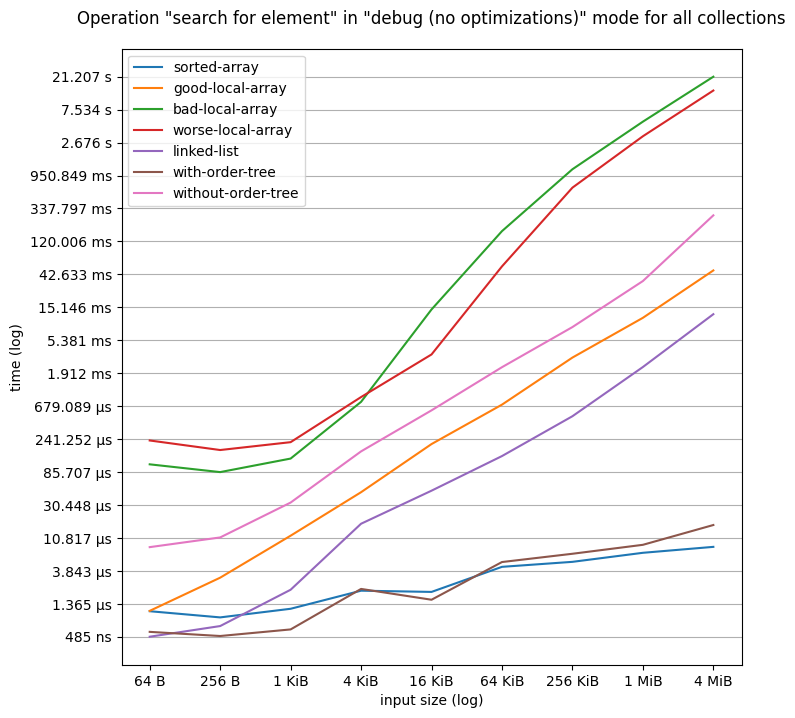
\includegraphics[width=15cm, keepaspectratio]
        {../charts/collections-find-debug.png}
    \end{center}
    \caption{Operação \textit{find} no modo ``\textit{debug}''
        (sem otimizações) para todas estruturas de dados}
    \label{fig:collection find debug}
\end{figure}

\begin{figure}
    \begin{center}
        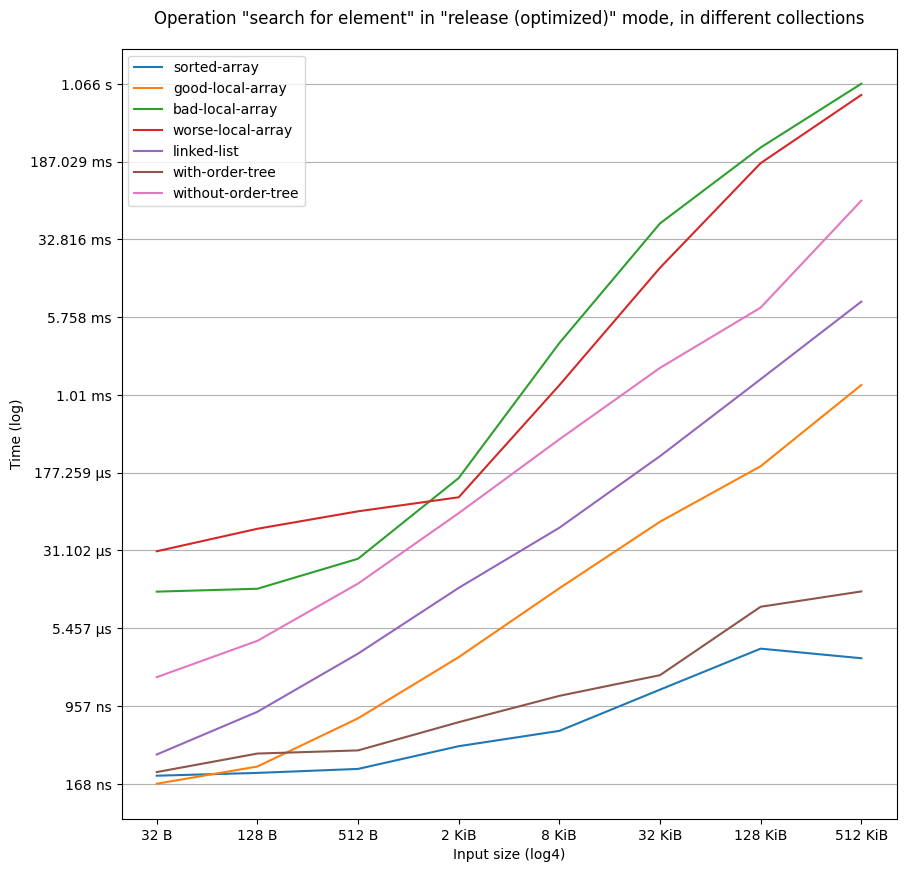
\includegraphics[width=15cm, keepaspectratio]
        {../charts/collections-find-release.png}
    \end{center}
    \caption{Operação \textit{find} no modo ``\textit{release}''
        (com otimizações) para todas estruturas de dados}
    \label{fig:collection find release}
\end{figure}

\begin{figure}
    \begin{center}
        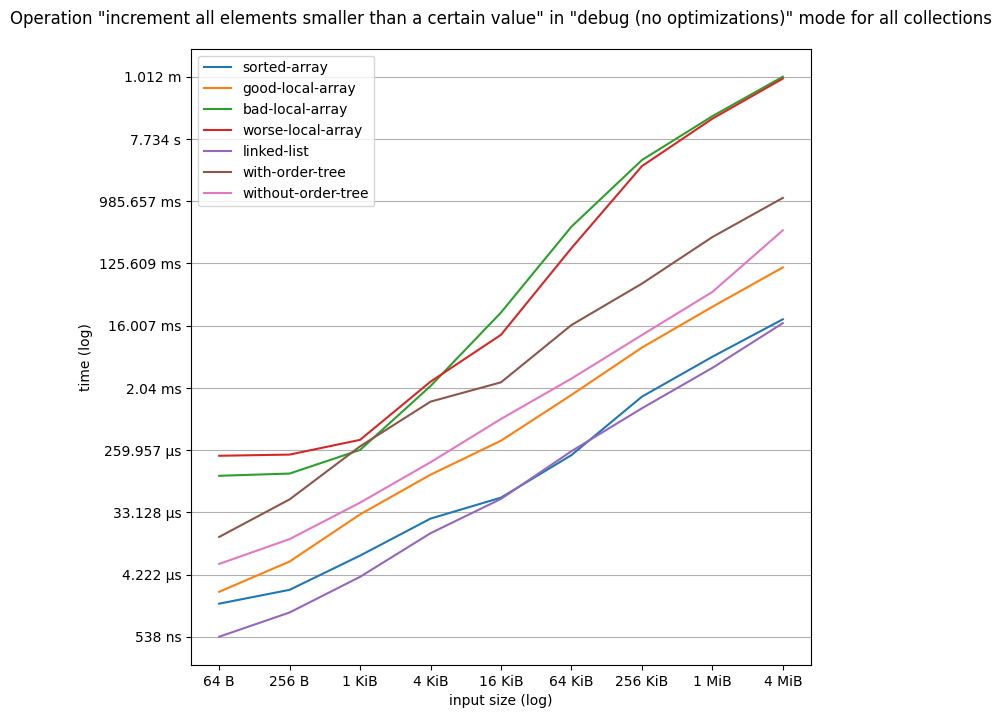
\includegraphics[width=16cm, keepaspectratio]
        {../charts/collections-inc-less-than-debug.png}
    \end{center}
    \caption{Operação \textit{inc less than} no modo ``\textit{debug}''
        (sem otimizações) para todas estruturas de dados}
    \label{fig:collection inc less than debug}
\end{figure}

\begin{figure}
    \begin{center}
        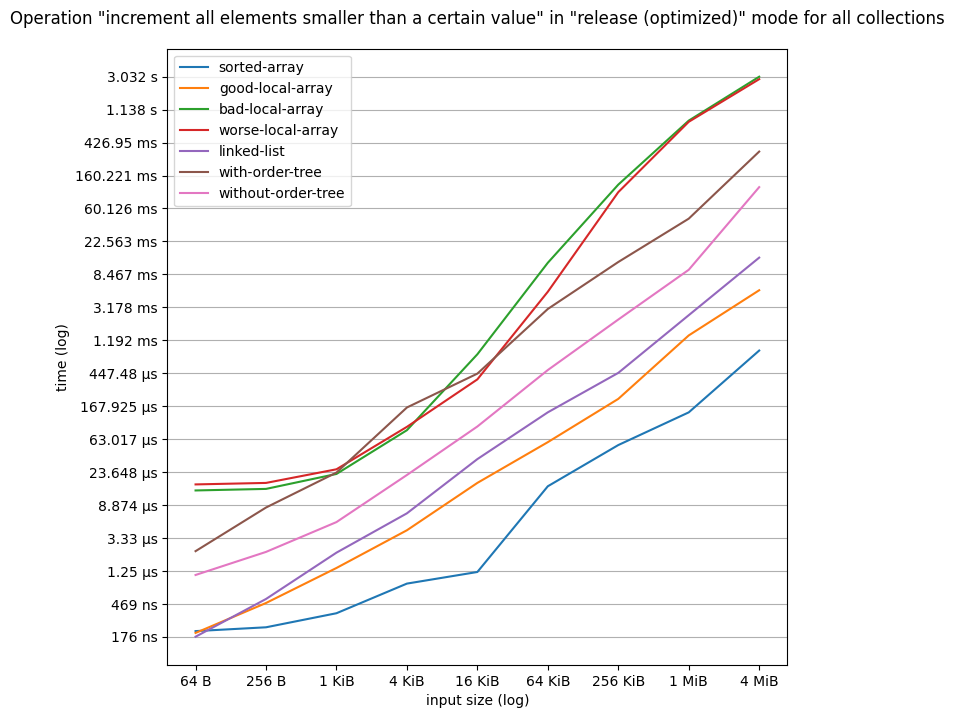
\includegraphics[width=16cm, keepaspectratio]
        {../charts/collections-inc-less-than-release.png}
    \end{center}
    \caption{Operação \textit{inc-less-than} no modo ``\textit{release}''
        (com otimizações) para todas estruturas de dados}
    \label{fig:collection inc less than release}
\end{figure}

Observando-se o gráfico da figura \ref{fig:collection find release},
observa-se que a ordenação na árvore binária é sim uma grande vantagem para
a operação de busca \textit{find}, ao comparar-se a versão com ordenamento e a
sem ordenamento. No entanto, para a operação \textit{inc-less-than}, na figura
\ref{fig:collection inc less than release}, observa-se que as duas versões da
árvore tiveram performance bastante similar, e apesar da versão com ordenamento
ter se saído um pouco melhor, não é algo significativo, e então, nessa operação,
o ordenamento não aparenta trazer vantagem.

Pode-se dizer que até há uma pequena vantagem ao usar ordenamento em árvores,
na operação \textit{inc-less-than}, com entradas de tamanho até
$16 KiB$, mas a partir de $64 KiB$, a performance das duas árvores converge.
Possivelmente, isso ocorre porque com entradas maiores, a chance da árvore
navegar por nodos em endereços em diferentes páginas é maior.

Na figura \ref{fig:collection inc less than release}, também se pode notar que
as versões sem ordenação do \textit{array} )(\textit{good-local-array},
\textit{bad-local-array} e \textit{worse-local-array}) tiveram uma diferença
significativa de performance entre a versão \textit{good-} e as versões
\textit{bad-} e \textit{worse-}. Para $4MiB$, a versão \textit{good-} conseguiu
$5.431 ms$, enquanto a versão \textit{bad-} atingiu $2.865 s$, e a versão
\textit{worse-} atingiu $2.851 s$, e a diferença é consistente para os vários
tamanhos de entrada usados.

No entanto, percebe-se que entre a versão \textit{bad-} e a versão
\textit{worse-} não há tanta diferença, e inclusive, para alguns tamanhos de
entrada, a versão \textit{worse-} surpreendentemente performa com um pouco menos
de tempo que a versão \textit{bad-}. Isso se repete na figura
\ref{fig:collection find release}, onde em alguns casos a versão
\textit{worse-} tem um desempenho melhor de forma levemente considerável,
em relação à versão \textit{bad-}. A respeito desses dois \textit{arrays},
também é notável que a partir do tamanho de entrada $4KiB$ (uma página),
a curva do tempo desses fica mais íngreme.

A lista encadeada \textit{linked-list} parece ter tido uma performance
intermediária, e inclusive foi mais rápida que árvores ordenadas na operação
\textit{inc-less-than} (figura \ref{fig:collection inc less than release}). No
entanto, \textit{sorted-array} e \textit{good-local-array} ainda superaram a
lista encadeada. É bom notar, contudo, que aqui se fala da execução com
otimizações ligadas, porém, sem otimizações (\textit{debug}), as listas
encadeadas superam \textit{good-local-array}
(figura \ref{fig:collection find debug}).

\FloatBarrier

\section{Considerações Finais}

Algumas conclusões interessantes podem ser feitas. Por exemplo, a partir do
resultado de \textit{bad-local-array} e \textit{worse-local-array}, pode-se
concluir que, se as páginas já estão sendo saltadas em uma grande quantidade
($16$ no nosso caso), não faz muita diferença intercalar entre duas metades de
um \textit{array} ou não, diferente do esperado. Uma explicação para tal é
que o TLB do sistema não leva em conta a proximidade das páginas, na verdade,
a vantagem está em endereços próximos em uma mesma página.

Além disso, pode-se verificar que, apesar do \textit{sorted-array} saltar entre
endereços muito distantes, a complexidade logarítimica da busca binária
compensa, porque a quantidade de endereços visitados é muito menor do que a
quantidade de endereços visitados por outros \textit{arrays}, por exemplo,
que podem acabar vasculhando todos elementos. Na verdade, uma observação
interessante é que a distância dos endereços da busca binária diminui a cada
iteração, porque a janela da busca diminui, então não ocorrem tantos saltos de
páginas como o esperado.

Outro fato interessante é que a vantagem de uma árvore ordenada sobre uma
árvore não-ordenada diminui e torna-se quase nula à medida em que se aumenta o
número de páginas em função do tamanho da entrada na operação de incremento.
É tentador associar isso à ideia de que a complexidade do algoritmo pode ser
irrelevante diante de uma alta quantidade de \textit{page misses} na TLB, mas na
realidade as duas complexidades não estão muito distantes: $O(max(m, n+m))$ versus
$O(n + m)$, onde $n$ é o tamanho da árvore, $m$ é o valor solicitado, e contam
como passos cada iteração.



\nocite{*}
\printbibliography

\end{document}
